\documentclass[AutoFakeBold]{article}
\usepackage{ctex}
\usepackage{geometry}
\geometry{left=2.5cm,right=2.5cm,top=3.0cm,bottom=2.5cm}
\title{大物作业}
\author{张博涵-应化1903(学号:1912020312)}
\date{\today}
\usepackage{graphics} 
\usepackage{listings}
\usepackage{framed}
\usepackage{amsthm,amsmath,amssymb}
\usepackage{wrapfig}
\usepackage{graphicx}
\usepackage{subfiles}
\usepackage{listings}
\usepackage{booktabs}
\usepackage{graphicx,times}
\usepackage{subfigure}         
\usepackage{natbib}
\usepackage{amssymb,amsmath}
\usepackage{geometry}
\usepackage{xcolor}
\usepackage{setspace}
\usepackage{subfigure}
\usepackage{physics}
\usepackage{array}
\usepackage{mhchem}
\begin{document}
\maketitle

\section{Question1}
\subsection{ }
以无限长直导线电流方向为z 轴正方向;$\displaystyle\va{\ce{MN}}$为 y 轴建立如下图所示的坐标系:

\begin{center}
\begin{figure}[h]
	\centering
	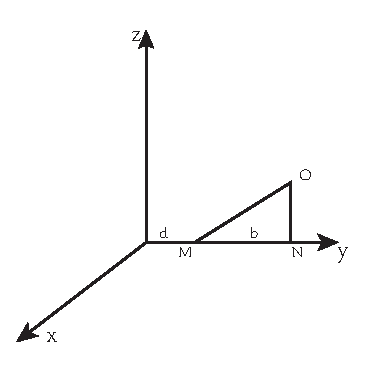
\includegraphics[scale = 0.7]{f1}
	\caption{Question1}
\end{figure}
\end{center}
此时取 MO 上的一点L($0,y,z$),其沿$\va{\ce{MO}}$的长度微小增量 d$\vec{l}$$ = (0,\ce{d}y,\ce{d}z)$。

无限长直导线在点L 处产生的磁场对应的磁感应强度$\va{B} = (-\dfrac{\mu_0 I}{4\pi y},0,0)$;根据题意,该点的速度为$\vec{v} = \left(\begin{array}{c}
	0\\
	0\\
	v
\end{array}\right)$。所以$\va{MO}$对应的感应电动势即动生电动势为:
\begin{align*}
			\int_{\va{MO}} (\vec{v} \times \va{B} )\cdot \ce{d}\vec{l} & = \int_{\va{MO}} ( \left(\begin{array}{c}
	0\\
	0\\
	v
\end{array}\right) \times (-\dfrac{\mu_0 I}{2\pi y},0,0) )\cdot(\ce{d}x,\ce{d}y,0)\\
& = -\int_{\va{MO}}\dfrac{\mu_0 Iv}{2\pi y}\ce{d}y = -\int_{d}^{d+b}\dfrac{\mu_0 Iv}{2\pi y}\ce{d}y =- \dfrac{\mu_0 Iv}{2\pi }\ce{ln}\frac{d+b}{d}
\end{align*}
由于$\dfrac{d+b}{d} = 1+\dfrac{b}{d} > 1$,故在$\va{MO}$上产生的感应电动势为负。方向与$\va{MO}$方向相反即由 O 至 M,且大小为$\dfrac{\mu_0 Iv}{2\pi }\ce{ln}\dfrac{d+b}{d}$
\subsection{ }
同理可得,在$\va{MN}$上产生的感应电动势与在$\va{MO}$上产生的感应电动势大小相等,方向相反。并在线段 NO上不产生感应电动势,所以总感应电动势为 0。
\section{Question2}
以无限长直导线电流方向为z 轴正方向;垂直于 z 轴且指向O 点方向为 y 轴正方向建立如下图所示的坐标系:
\begin{center}
\begin{figure}[h]
	\centering
	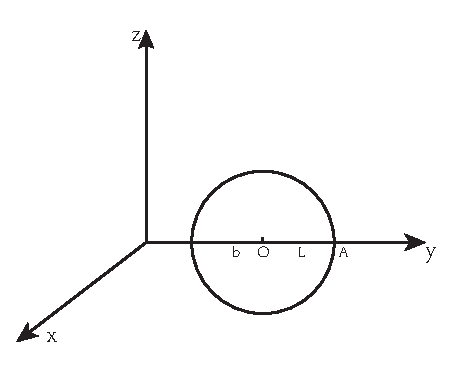
\includegraphics[scale = 0.7]{f2}
	\caption{Question2}
\end{figure}

\end{center}
取$\va{OA}$上一点(0,y,0),取其在 y 轴上的微小增量d$\vec{l} = (0,\ce{d}y,0)$


无限长直导线在点L 处产生的磁场对应的磁感应强度$\va{B} = (-\dfrac{\mu_0 I}{4\pi l},0,0)$;根据题意,该点的速度为$\vec{v} = \left(\begin{array}{c}
	0\\
	0\\
	\omega(y-L)
\end{array}\right)$。所以$\va{OA}$对应的感应电动势即动生电动势为:
\begin{align*}
			\int_{\va{OA}} (\vec{v} \times \va{B} )\cdot \ce{d}\vec{l} & = \int_{\va{OA}} ( \left(\begin{array}{c}
	0\\
	0\\
	\omega(y-L)
\end{array}
\right) \times (-\dfrac{\mu_0 I}{2\pi y},0,0) )\cdot(0,\ce{d}y,0)\\
 & = -\int_{\va{OA}}\dfrac{\mu_0 I\omega(y-L)}{2\pi y}\ce{d}y = -\int_{b}^{b+L}\dfrac{\mu_0 I\omega(y-L)}{2\pi y}\ce{d}y\\
 & = -\dfrac{\mu_0 I\omega}{2\pi }(L-b\ce{ln}\frac{L+b}{b})
\end{align*}
由图可知,上面算出的感应电动势是负的,说明其方向与$\va{OA}$相反,即 A 点电势高,且感应电动势大小为$\dfrac{\mu_0 I\omega}{2\pi }(L-b\ce{ln}\dfrac{L+b}{b})$。
\end{document}